\documentclass[letterpaper, 11 pt, proceedings]{IEEEtran}
\usepackage{amsmath}
\usepackage[margin=.65in]{geometry}
\usepackage{enumitem}
\usepackage{float}
\usepackage{graphicx} % Required for inserting images
\usepackage{helvet}
\usepackage{hyperref}
\usepackage{listings}
\usepackage{mathptmx}
\usepackage{nameref}
\usepackage{pgfplots}
\usepackage{placeins}
%\usepackage{subcaption}
\usepackage{titlesec}
%\usepackage{wrapfig}
%\renewcommand{\familydefault}{\sfdefault}
\graphicspath{{./figures/}}

%\titlespacing*{\section}{0pt}{0.5\baselineskip}{0.25\baselineskip}
%\titlespacing*{\subsection}{0pt}{0.5\baselineskip}{0.25\baselineskip}
%\titlespacing*{\subsubsection}{0pt}{0.5\baselineskip}{0.25\baselineskip}

\titlespacing*{\section}{0pt}{0.5\baselineskip}{0.2\baselineskip}
\titlespacing*{\subsection}{0pt}{0.25\baselineskip}{0.25\baselineskip}

% Abstract
% Introduction: The goals of the project, the motivation, and the approach used.
% Background: Summary of important concepts and related previous work (with citations).
% Methods: Detailed description of the methods used, including equations, algorithms, rules, etc. and a justification for the approach.
% Results: Description and discussion of results, with figures, tables, etc.
% Conclusion: Summary of accomplishments, challenges and open issues.
% Bibliography: Full list of all papers cited in the report in paper, consistent format




\title{Exploring Stock Market Strategies with Risk and Influence with Complex Networks}
\author{Rachael Judy, Connor Klein, Josh Smith}
\date{21 April 2024}

\begin{document}
	\pgfplotsset{compat=1.18}
	\setlist[itemize]{noitemsep}
	\setlist[enumerate]{noitemsep}
	
	\maketitle

	\begin{abstract}
		This paper explores the impact of risk strategies and influenced decisions in a complex network of brokers, simulating the stock market over different intervals. Using fat-tailed distributions for risk evaluation and friend count, it demonstrates how some risk strategies can perform well over typical behavior of the market while others can benefit from sudden volatile events. It also explores how the influence of a broker's neighbors on the risk assessment can affect brokers' portfolio values. 
	\end{abstract}


	\section{Introduction}\label{sec:intro}
	% Introduction: The goals of the project, the motivation, and the approach used.
	The volatility of economic markets is a popular area of study for many researchers, and markets have been shown to contain many fat-tailed distributions and power laws, such as in growth rates and stock returns \cite{gabaix_powerlaws}. Scholars have examined risk and its aversion, modeled the market as a network of stocks or brokers, attempted to classify and group cliques within the network, and designed models of real-world crashes. This project combines the spread of individual risk adversity, a fat-tailed distribution of network connections, and theory on different strategies in volatile \cite{taleb_antifragile} events with the goal of evaluating broker strategies for maximizing portfolio value over typical events and through drastic changes in the market. This is explored through a simulation over different market intervals using the assumptions of complex networks and fat-tailed distributions from previous research.
	
	Section \ref{sec:background} discusses background and assumptions, \ref{sec:methods} explains the simulation design, \ref{sec:results} highlights key results, and \ref{sec:conclusion} overviews the results and future work.
	
	\section{Background}\label{sec:background}
	% Background: Summary of important concepts and related previous work (with citations).
	Financial markets have been explored from a variety of fields, such as psychology, economics, statistics, graph theory, and complex systems. Each of these fields explores various aspects of the market  from modeling in terms of complex networks of agents and entities in the market, looking at individuals' and groups' perspective on risk, and running case studies with different clustering and strategies in the market. Within complex networks, the networks place either brokers or stocks at the nodes \cite{baydelli_hierarchicalmarket,kulmann_marketscomplexsystems,dimaggio_relevancebrokernetworks,tse_networkstocks}. For the edges of the network, the diffusion of information \cite{dimaggio_relevancebrokernetworks}, spread of first and rebound shocks \cite{gai_contagion}, and correlation and mutual information of different stocks \cite{li_correlation, fiedor_networksmutualinformationrate} have been evaluated. This study models the market with brokers at the nodes with influence on risk adversity connecting the brokers. 
	
	Further, several models for risk have been explored. These studies include quantifying the risk with the Chen, Roll, and Ross factors \cite{cooper_realinvestmentandrisk} to predict economic activity, assessing the importance of the distribution of risk aversion in the volatility of returns \cite{lansing_riskaversion}, and highlighting the importance of dividends in quantifying the risk level of stocks. These models provide a basis for developing a model of portfolio risk.
	
	Additionally, based on the ideas presented in Taleb's book \cite{taleb_antifragile}, it has been suggested that some strategies which perform well over typical market moves may not be optimal during sudden volatile events in the fat-tailed distribution of stock market prices and behavior. Using strategies based on risk allows exploration of different levels of fat-tailed risk adversity and the impact of networked brokers sharing information about risk on portfolio value during both expected operation of the market and the aforementioned Black Swan events.
	
	
	\section{Methods}\label{sec:methods}
	% Methods: Detailed description of the methods used, including equations, algorithms, rules, etc. and a justification for the approach.
	The project was designed as a simulation to be run over various time intervals for interconnected brokers that can influence one another and with individual preferred risk levels. $n=100$ brokers were created, each with a preferred risk level and a number of friends sampled from a power law distribution. The details of these selections are highlighted in the following subsections. The friends' assessments of the risk of a given stock are then used by the broker in their personal assessment. Data for every day in the interval is fed into the simulation, allowing brokers, in a random order, to buy or sell stocks to maintain their preferred level of risk. Another option is for brokers to hold their portfolio until the end of interval once preferred risk is achieved. For the ease of interpretation of results, the brokers' indices correspond to the level of preferred risk. For this paper, the simulation was run over 2003-2012, allowing examination of the results of strategies both in normal operating conditions and in drastic events such as the 2007-2008 financial crisis.
	
	\subsection{Data Collection and Filtering}\label{subsec:data}
	The available tickers were collected from Yahoo Finance's API \textit{yfinance}. Valid stock tickers were pulled that contain daily stock information at any point from the time period of 2000 to 2020, totaling 10,000 individual tickers. These tickers were filtered to those with the information needed for the risk calculation discussed in section \ref{subsec:risk}, and 175 stocks were randomly selected from those options to be fed into the simulation. This limitation was imposed to only include stocks with necessary information and to not exceed a reasonable time frame for running the simulation. This data was then stored in a Pandas dataframe for quick accessibility by the simulation at runtime.
	
	For these stocks, missing price data was set to the most recent value from the time series. Certain values such as dividend rate and estimated earnings per share were available only as single values instead of time series; this API limitation creates some inaccuracy in our risk calculation as these single values would fluctuate over time. There is the additional limitation of Yahoo finance not recording tickers that take their ticker off the public stock market, for reasons such as bankruptcy or private buyout.
	

	\subsection{Influence and Friend Selection}\label{subsec:friends}
	The number of friends for each broker was selected with a fat-tailed distribution with $\alpha = 2.7$ and a minimum value of $2$ friends. This distribution was chosen to mimic the number of connections a given person has. The selection of that number of friends for set of friends F was than randomly chosen from a uniform distribution over all the possible brokers. These connections for influence were directed, giving each broker the given number of inputs on the risk assessment. Further, each friend started with a set percent $w_i = .04$ controlled of the broker i's risk assessment. Thus, the risk for a stock $s$ is represented with the formula:
	\begin{align}
		R(\text{s}) = (1-\sum\limits_{f\in F} w_f) R_{broker}(\text{s}) + \sum\limits_{f\in \text{F}} w_f R_f(\text{s}).\label{eq:weighted_assessment}
	\end{align}	
	
	The influence of each friend providing input is increased or decreased based on its own gains or losses compared to the broker being advised. If a broker's neighbor's portfolio improved relative to broker's status, that neighbor is given more influence on the next risk assessment.

	\subsection{Risk Calculation}\label{subsec:risk}
	The risk for an individual stock was calculated using the formula with a exponential representation of $R_f(s) = ax^{-k}$ with:
	\begin{align}
		x &= e^{|H_{52} - L_{52} - d_r \times m_{50}|} \\
		a &= p_a \times f_{eps} \times (1 - e_g)\\
		k &= 3
	\end{align}

%	\begin{align}
%	\[a \cdot x^{-k}\]\text{where:}
%		\[
%		x = e^{\left| \text{{high}} - \text{{low}} - \text{{dividend\_ratio}} \times \text{{fifty\_day\_average}} \right|}
%		\]
%		\[
%		a = \text{{portfolio\_allocation}} \times \text{{forward\_eps}} \times (1 - \text{{earnings\_growth}})
%		\]
%	\end{align}
	
	The risk is represented by a fat-tailed distribution with an exponent of $k=3$ with $H_{52}$ as the 52-week high, $L_{52}$ as the 52-week low, $d_r$ as the dividend ratio, $m_{50}$ as the 50 day average, $e_g$ as the earnings growth, $f_{eps}$ as the forward earnings per share, and $p_a$ as the portfolio allocation of equity for the given stock. 
	
	Within this formula based on research on risk, $a$ represents the likelihood of risk to have major effects while $x$ is the representation of the potential impact of the stock, capturing the volatility of the stock minus an expected return. This value is an exponential so that it remains in the range $[1, \infty)$.
	The product of these values represent the risk of the stock. The portfolio risk is then the sum of each individual stock risk multiplied by the volume in the portfolio. In the simulation, the numerical values of risk from 0 to 10000 were linearly spread over the brokers. Brokers seeking to raise their risk level sell lower risk stocks and purchase from the riskier stocks evaluated with equation \ref{eq:weighted_assessment}.

	\begin{figure}[h]
		\centering
		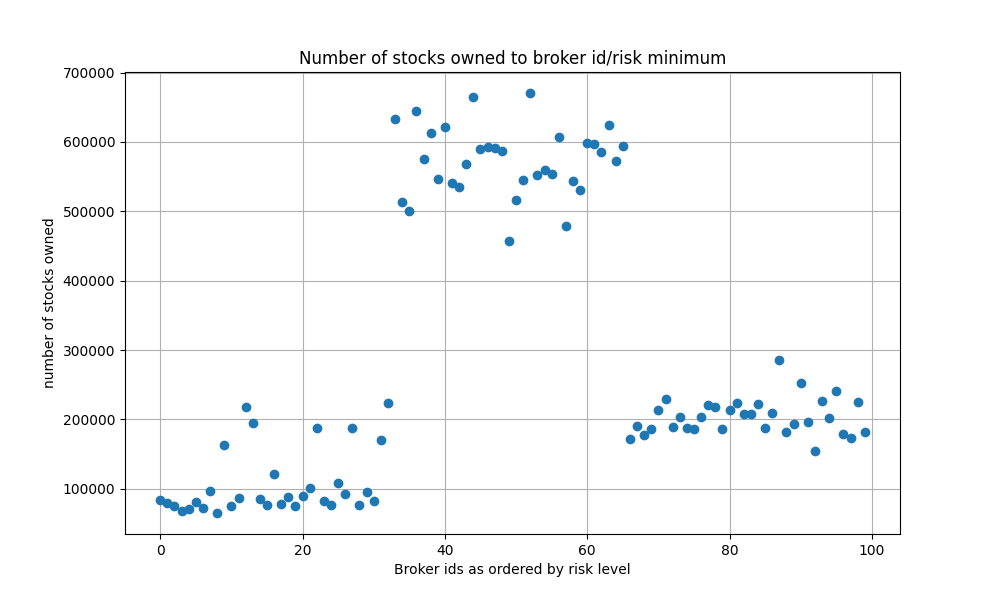
\includegraphics[width=0.5\textwidth]{stocksOwnedToBrokerIds.png}
		\caption{Total number of stocks owned by broker id (corresponding to risk level)}
		\label{totalvID}
	\end{figure}
	
		
	\subsection{Metrics}\label{subsec:metrics}	
	The portfolio value $V(b_i)$ at any point in time is represented as the sum of the liquid money $m_i$ the broker $b_i$ has and the current value $v_s$ multiplied by the quantity $q_s$ of every stock owned by the broker at the given time: 
	\begin{align}
		V(b_i) = m_i + \sum\limits_{s\in\text{stocks}} v_s q_s\label{eq:portfolio_value}
	\end{align}
	The portfolio risk, quantified by section, \ref{subsec:risk} represents the level of risk each broker attempted to maintain while the portfolio value at different times in the interval was used to evaluate the strategy's overall performance.

	\section{Results}\label{sec:results}
	% Results: Description and discussion of results, with figures, tables, etc.
		
	% risk results
	% Hopefully useful thoughts:
	% - possibly include quick overview showing that high risk brokers tend to own few stocks total of higher value while ones in the middle show the more typical lots of stocks, and most conservative end up with less stocks and more liquid - requires figure of money at end, stock quantity to broker, and liquid money to broker
	% - focus in on a point before 2008 and which level of risk broker is doing well in the wealth time series and then who is doing well after the crash ie high risk
	% - examine immediately after crash wealth v in couple years after
	% - for the case of stop_at_stable and not stop_at_stable, highlight differences in just sitting once at the desired risk v holding the desired risk by buying and selling
	
	\subsection{Broker Tendencies Resulting from Risk Level}\label{subsec:tendencies}	
%	\begin{figure}[h]
%		\centering
%		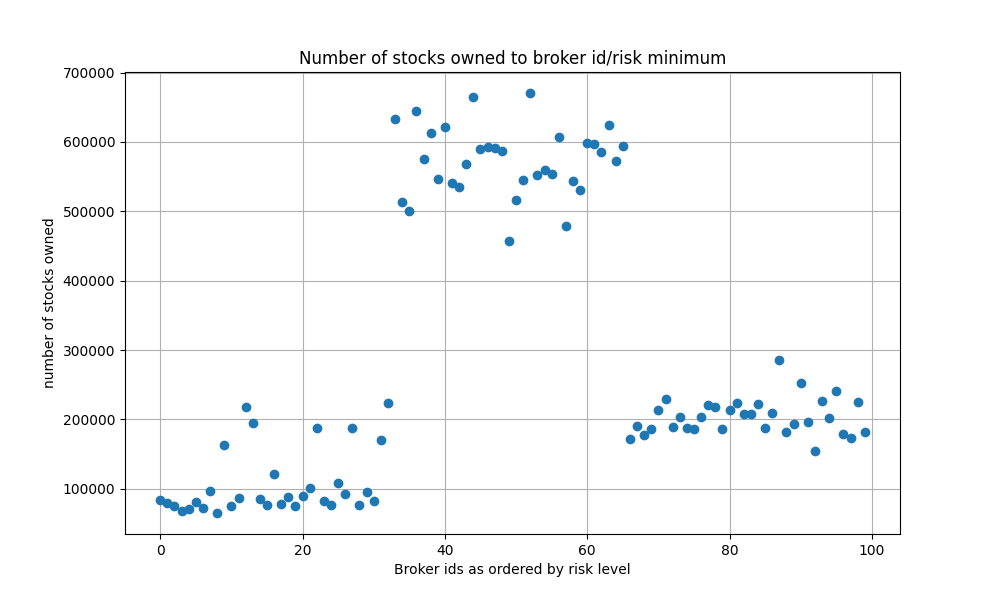
\includegraphics[width=0.5\textwidth]{stocksOwnedToBrokerIds.png}
%		\caption{Total number of stocks owned by broker id (corresponding to risk level)}
%		\label{totalvID}
%	\end{figure}
	\begin{figure}[h]
		\centering
		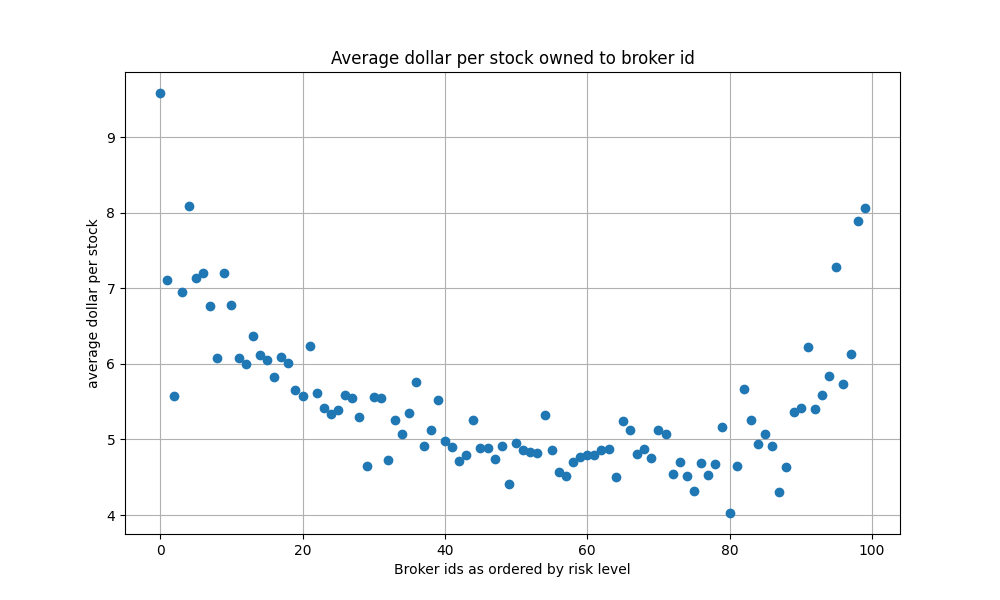
\includegraphics[width=0.5\textwidth]{averageDollarPerStockToBrokerIds.png}
		\caption{Average dollar value of stock owned to broker id (corresponding to risk level)}
		\label{dollarValue}
	\end{figure}
	\FloatBarrier
	As discussed in section \ref{sec:methods}, the Broker index/id corresponds to its relative desired risk level. The portfolio data compared to these risk levels show certain results of a given risk. These statistics include the total quantity of stocks in portfolio, the average value of stocks owned by a broker, and the value of liquid assets over time.
		
	\begin{figure}[h]
		\centering
		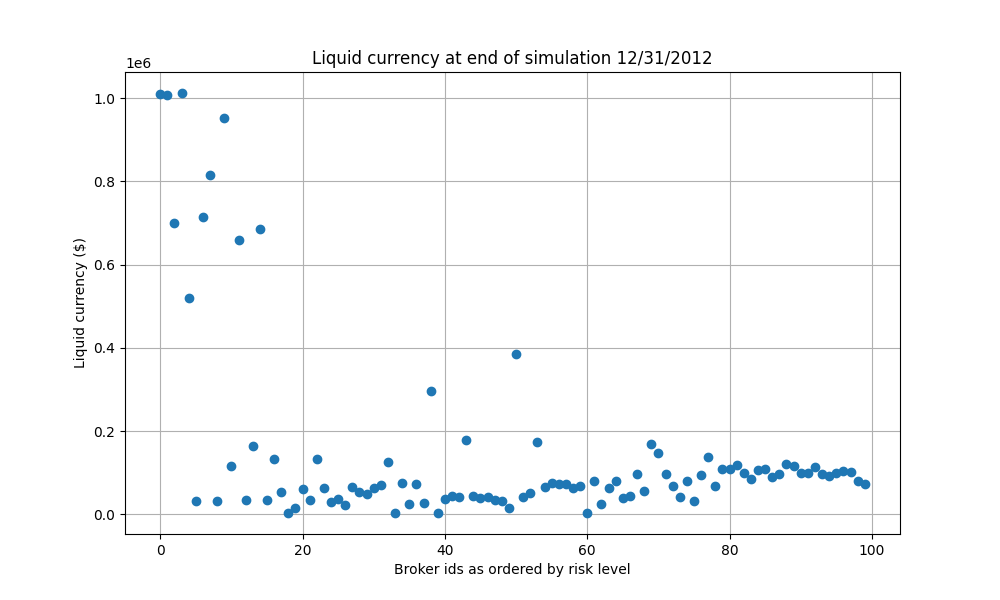
\includegraphics[width=0.5\textwidth]{liquidCurrency.png}
		\caption{Liquid currency at end of simulation vs broker id (corresponding to risk level)}
		\label{liquidvID}
	\end{figure}
	\FloatBarrier	
		
	Figure \ref{totalvID} shows that both low-risk and high-risk brokers tend to own few stocks compared to that of medium-risk brokers. This ownership appears to be parabolic with a flat curve defining the maximum. Looking at Figure \ref{dollarValue} in connection to the total stocks owned shows that high risk brokers tended to own a small number of expensive stocks while medium risk brokers acquire more low value stocks. The high volume ownership of expensive stocks, as expected, was evaluated as a more risky portfolio as putting all money on a specific stock risks the entire portfolio failing on that stock.

%	The two ends of this curve are explained in Figure \ref{uniquevID}. Here, the levels at which unique stocks are owned are inverted compared to Figure \ref{totalvID}. 
	
%	Both risk-averse and risky brokers tend to own a number of unique stocks, while those with medium risk tend to own more of the same type of stocks. The ownership of multiple stocks in different industries can be seen as less risky, as owning more individual stocks allows certain investments to fail without affecting the total as much. This is compared to a high ownership of a specific stock, which, if it goes under, results in the entire portfolio going under as well. 

%	\begin{figure}[h]
%		\centering
%		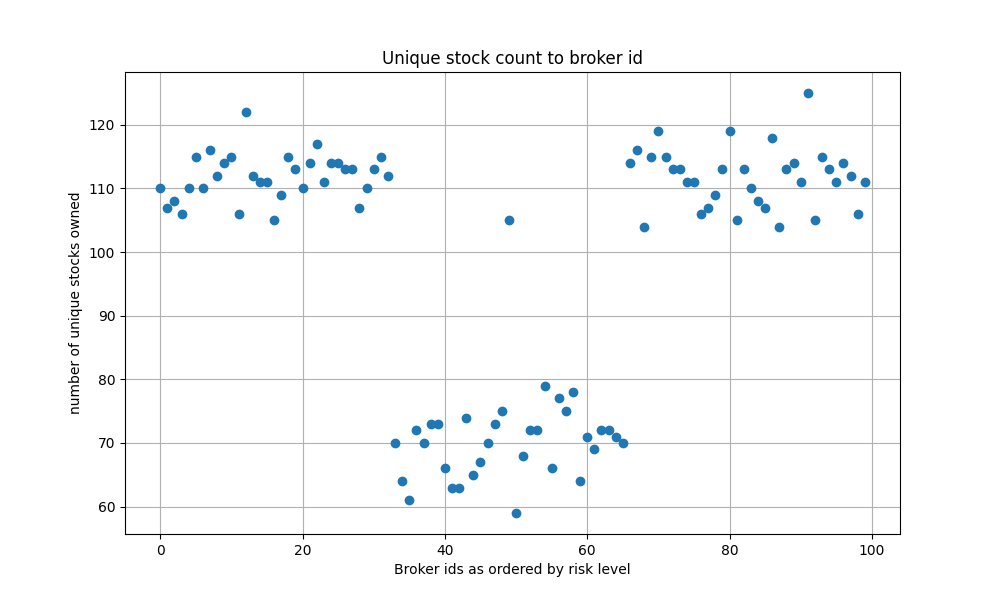
\includegraphics[width=0.5\textwidth]{uniqueStockCountToBrokerIds.png}
%		\caption{Unique stocks owned by Broker Id}
%		\label{uniquevID}
%	\end{figure}
%	\FloatBarrier


	Further, the liquid currency of each broker at the end of the interval expands the picture of the differing investment strategies of low and high-risk investors. Figure \ref{liquidvID} shows that risk-averse brokers tend to keep as much as 100\% of their assets liquid, meaning they are not invested in the market and their portfolio values can remain stable. Meanwhile, higher risk brokers tend to invest most of their assets into the market.
	
	These three aspects of quantity of stocks owned, average stock value, and currency show the behaviors of different brokers based on their desired levels of risk.

	\subsection{Market Strategies Over Time}\label{subsec:results_midpoint}
	The simulation was run over the period from the beginning of 2003 to the end of 2012, capturing the 2007-2008 financial crisis as well as some expected behavior of the market. It is beneficial to analyze how different risk strategies performed with and without the Black Swan event to determine if certain strategies are better given the goal of developing an antifragile strategy. Figure \ref{interimRV} shows that pre-2008, both high and medium-risk strategies were outperforming low-risk strategies. However, the most risky brokers were underperforming compared to the medium risk brokers in typical operation. It is important to note that all brokers were able to increase their portfolio value over this time.

	\begin{figure}[h]
		\centering
		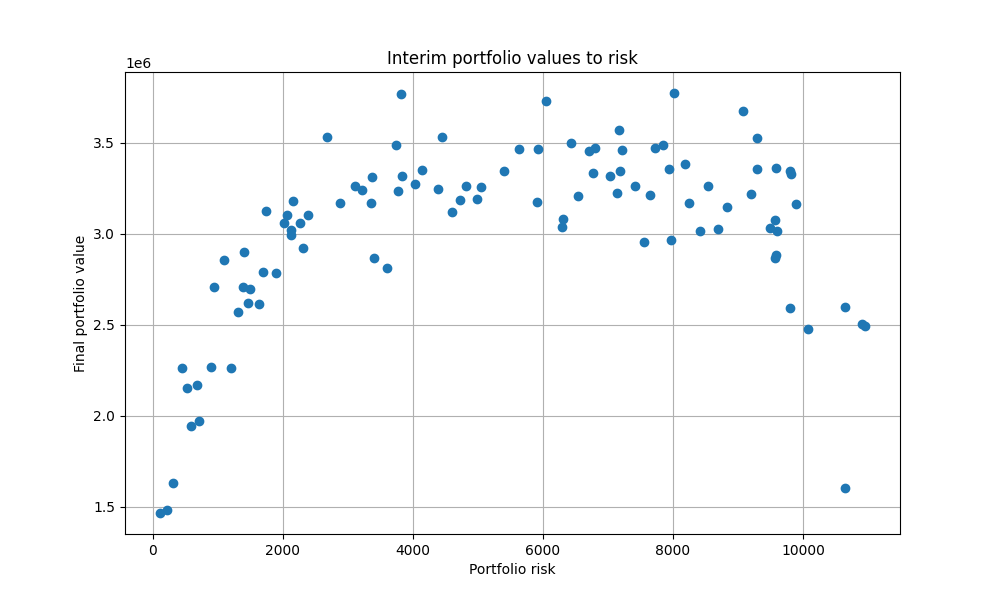
\includegraphics[width=0.5\textwidth]{interimRiskToValue.png}
		\caption{Value of portfolios before Black Swan event}
		\label{interimRV}
	\end{figure}
	\FloatBarrier

	\subsection{Antifragile Strategies}\label{subsec:results_end}	
	
	Figure \ref{ts_03-12} shows some examples of the wealth of brokers with different strategies throughout the simulation. The total wealth of the brokers' assets all appear to follow the general market trends and grow over time. All of the brokers experienced a significant loss when the 2007-2008 financial crisis occurred; however, the brokers, who did not cash out when the stocks crashed, rebounded after the crisis. By 2010, the typical brokers regained the wealth that they had acquired before 2008. The high risk brokers can be seen to rebound more quickly and exceed their peers of medium risk in some cases. Further, it showed buying at the crash showed significant increase in portfolio value for brokers seeking medium and high levels of risk.
	
	\begin{figure}[h]
		\centering
		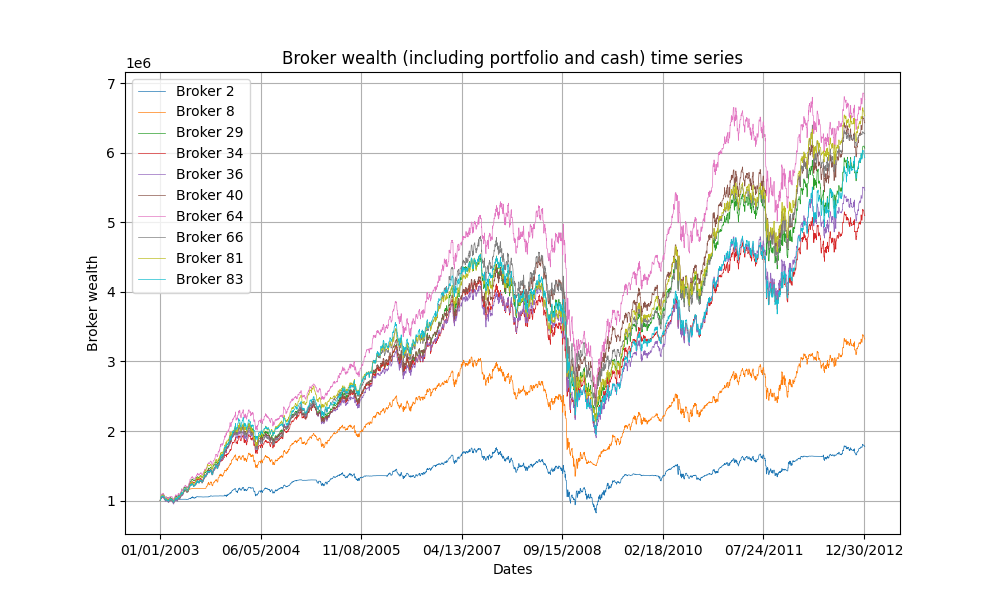
\includegraphics[width=0.5\textwidth]{timeSeriesJoint2.png}
		\caption{Time series of selected brokers' wealth with ids corresponding to risk level}
		\label{ts_03-12}
	\end{figure}
	\FloatBarrier


	\begin{figure}[h]
		\centering
		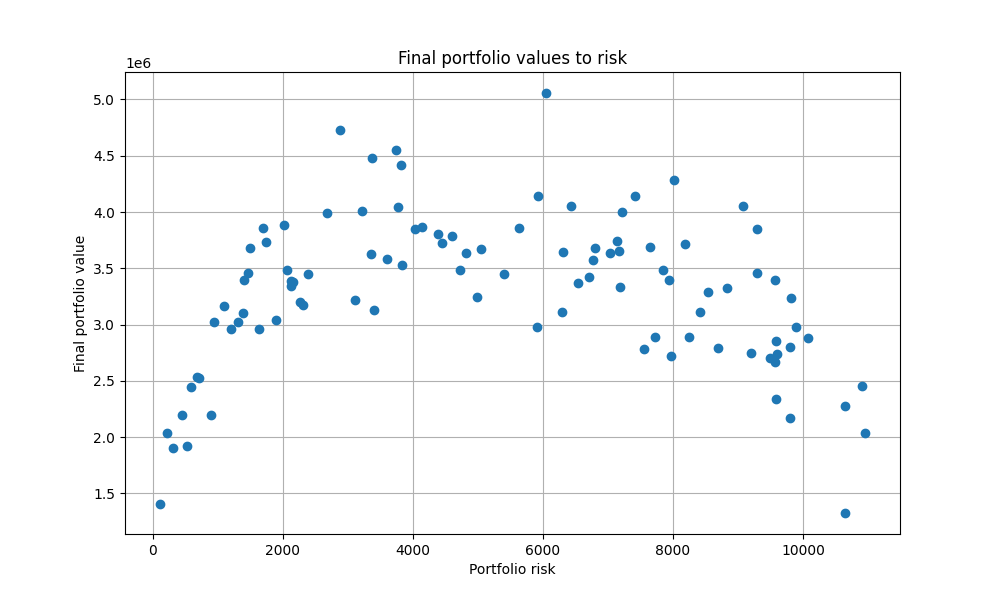
\includegraphics[width=0.5\textwidth]{valueToRisk.png}
		\caption{Value of portfolios at end of simulation ordered by broker ids which correspond to risk level}
		\label{RV}
	\end{figure}
	\FloatBarrier

	As occurred under normal conditions in Figure \ref{interimRV}, the medium-risk brokers appeared to have acquired the most wealth. However, comparing the final values shows a slightly different behavior as in Figure \ref{RV}. High-risk brokers, by not exiting when their portfolios spiked, did not achieve the same levels of wealth as the more moderate brokers after the Black Swan event. The curve in Figure \ref{RV} is very parabolic, where both the low and high-risk brokers did not acquire as much wealth as the moderate-risk broker. This is in comparison to Figure \ref{interimRV}, where the curve flattens and stays flat, indicating that high-risk brokers also perform well.
	
	Additionally, simulations were performed where once a broker accomplished their desired risk, they would stop investing. This was to simulate a real-world strategy of investing and sitting on the portfolio. Brokers, although starting with the same risks as in other simulations, ended up becoming less risky by the end of the simulation. Figure \ref{stopatstable} shows that most portfolios became less stable without input from the brokers. This is in comparison to Figure \ref{RV}, where the distribution of risk remains consistent as was initialized. It is also important to note that brokers maintaining their investments performed similarly to brokers who continuously invested after the Black Swan event.

	\begin{figure}[h]
		\centering
		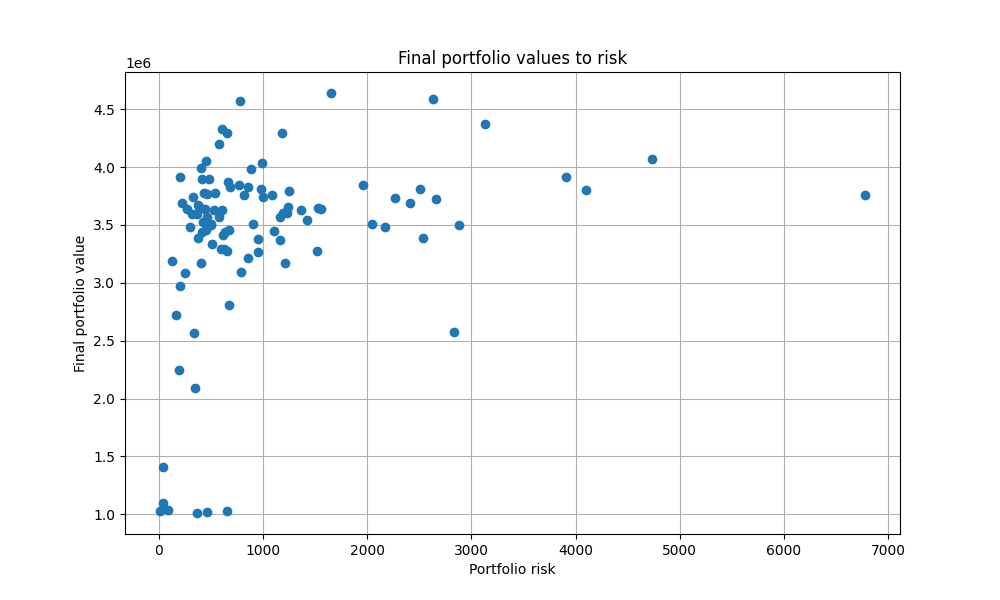
\includegraphics[width=0.5\textwidth]{valueToRisk_stopatstable.png}
		\caption{Portfolio values by risk when brokers stop at preferred risk level}
		\label{stopatstable}
	\end{figure}
	\FloatBarrier
	
	\subsection{Influence}
	% influence results
	% Seems like influence as is feeds into risk incorrectly because the only difference between the broker's assessment is really how much of that stock they own and its value in their portfolio
	% influence would be more relevant if partial information came into play instead of just how risky the broker wanted to be
	
	\begin{figure}[h]
		\centering
		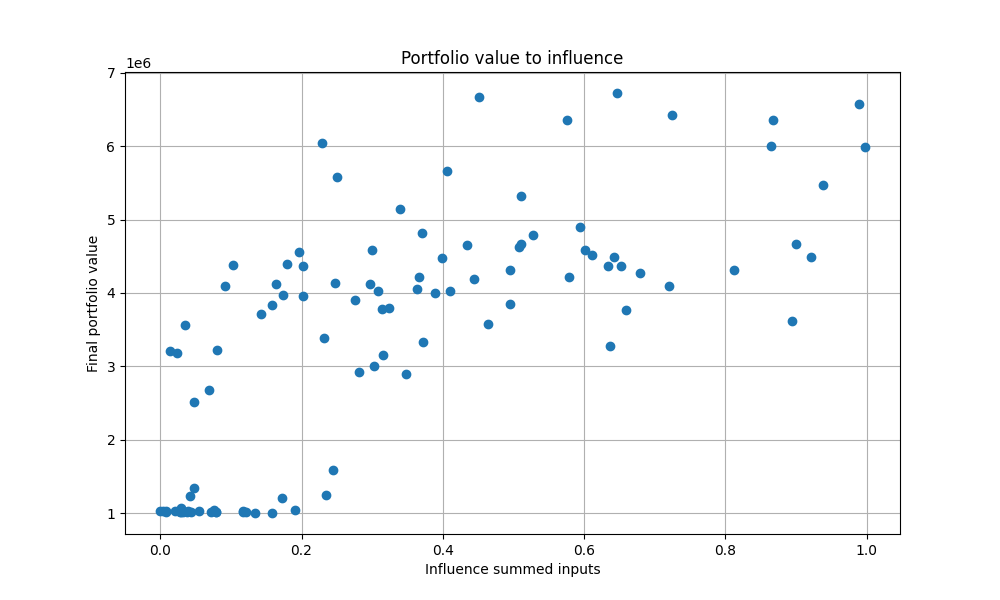
\includegraphics[width=.5\textwidth]{valueToInfluence_influence04.png}
		\caption{Plot of portfolio values to percent of decision made based on friends' recommendations on risk}
		\label{fig:value_to_influence_influencerun}
	\end{figure}	
	\FloatBarrier


	The simulation examining the impact of influence assigned the brokers to either a low, medium, or high risk level. Within each group, the brokers were ordered from lowest amount of initial friends to greatest quantity, sampled from the fat-tailed distribution discussed in \ref{subsec:friends}. The plot in Figure \ref{fig:value_to_influence_influencerun} shows that allowing a large 50-100\% portion of the purchase assessment to be made with input from neighbors improves the portfolio value. While there is a wide range of values at a given influence, it generally improves with up to around 50\% of the risk assessment being provided by friends. This is likely because taking multiple neighbors' input highlights stocks that are doing well for multiple different brokers, making the decision easier and capturing the change in value directly that the risk assessment did not capture. Further, it can be seen that this benefit of influence was consistent across the different risk levels by examining Figures \ref{fig:low_risk_influence_time_series} and  and \ref{fig:high_risk_influence_time_series}. Basing the influence connections of the network around the risk assessment provides an expansion on a single broker's understanding of the stocks behavior but did not entirely capture the additional benefit of accessing partial information as desired.
	
	\begin{figure}[h]
		\centering
		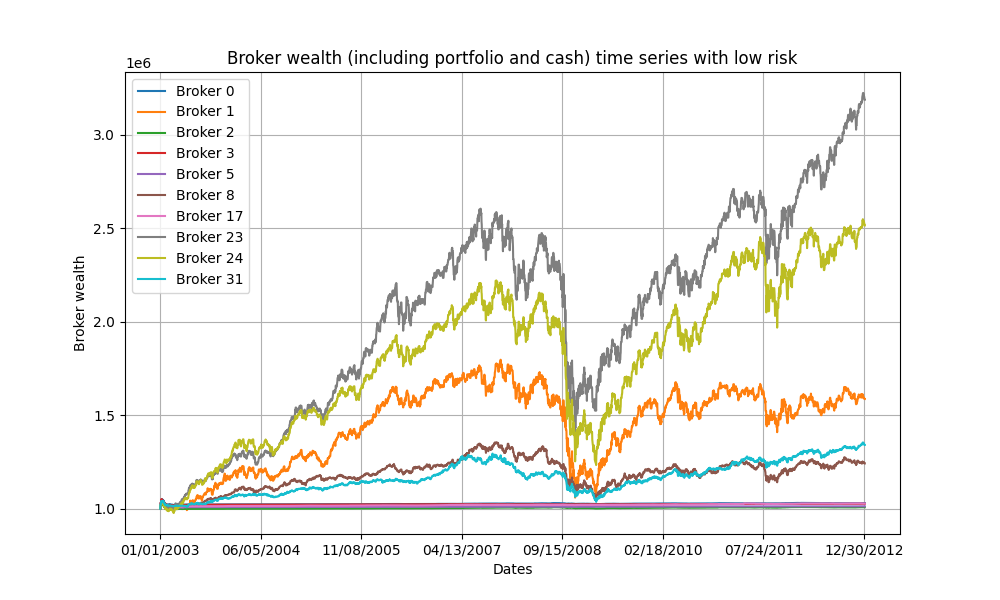
\includegraphics[width=.5\textwidth]{timeSeriesJoint_influenceRun04_LowRisk.png}
		\caption{Time series of portfolio values of brokers with low risk ordered by number of friends providing input on risk assessment for stock purchases}
		\label{fig:low_risk_influence_time_series}
	\end{figure}	
	\FloatBarrier
	
	\begin{figure}[h]
		\centering
		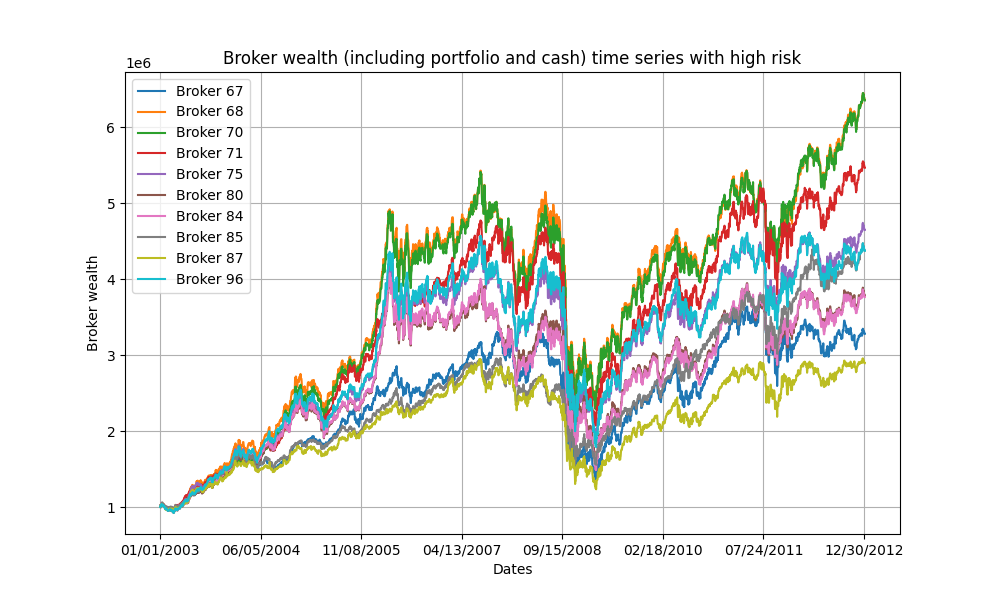
\includegraphics[width=.5\textwidth]{timeSeriesJoint_influenceRun04_HighRisk.png}
		\caption{Time series of portfolio values of brokers with high risk ordered by number of friends providing input on risk assessment for stock purchases}
		\label{fig:high_risk_influence_time_series}
	\end{figure}	
	\FloatBarrier
	
	
	\section{Conclusion}\label{sec:conclusion}
	% Conclusion: Summary of accomplishments, challenges and open issues
	This project explored the value of different risk strategies in a simulated market of networked brokers with power law assumptions for risk and connectivity between brokers. It demonstrated the value of taking some input from neighbors' assessments on risk to filter which stocks are performing well and showed that both risk adverse and risky market strategies underperform medium-risk strategies. Notably, during black swan events such as the 2008 financial crisis, low and high-risk strategies perform even worse compared to medium-risk strategies.
	
	\subsection{Future Work}\label{subsec:futurework}
	Given the scope of time for the project, only limited aspects of market strategies could be explored. One open area is expanding the concept of influence, as the method of all neighbors using the same information and formula acted as simply a factor of the risk calculation. Additionally, the random selection of neighbors may not capture the true clique structure of many relationships. Further, the risk assessment could be modified to vary more between brokers based on partial information and stocks without full information available in order to better represent the real world and account for the interconnections between stocks.


	\bibliographystyle{ieeetran}
	\begin{thebibliography}{99}	
		\bibitem{gabaix_powerlaws}
		X. Gabaix, “Power laws in economics: an introduction,” \textit{Journal of Economic Perspectives}, vol. 30, no. 1, pp. 185–206, Feb. 2016.
		
		\bibitem{taleb_antifragile}
		N. N. Taleb, \textit{Antifragile: Things that gain from disorder}. Harlow, England: Penguin Books, 2013.
		
		\bibitem{baydelli_hierarchicalmarket}
		Y. Y. Baydilli, S. Bayir, and I. Tuker, “A hierarchical view of a national stock market as a complex network,” \textit{Economic Computation \& Economic Cybernetics Studies \& Research}, vol. 51, no. 1, pp. 205–222, Jan. 2017.

		\bibitem{kulmann_marketscomplexsystems}
		M. Kuhlmann, "Explaining financial markets in terms of complex systems," \textit{Philosphy of Science}, vol. 81, no. 5, pp. 1117-1130, Dec. 2014. %doi: 10.1086/677699.
		
		\bibitem{dimaggio_relevancebrokernetworks}
		M. Di Maggio, F. Franzoni, A. Kermani, and C. Sommavilla, "The relevance of broker networks for information diffusion in the stock market," \textit{Journal of Financial Economics}, vol. 134, no. 2, pp. 419-446, Nov. 2019. %doi: 10.1016/j.jfineco.2019.04.002. 

		\bibitem{tse_networkstocks}
		C. K. Tse, J. Liu, and F. C. M. Lau, “A network perspective of the stock market,” Journal of Empirical Finance, vol. 17, no. 4, pp. 659–667, Sep. 2010.
		%- https://www.sciencedirect.com/science/article/pii/S0927539810000368

		\bibitem{gai_contagion}
		P. Gai and S. Kapadia, "Contagion in financial networks," \textit{Proceedings of the Royal Society}, vol. 466, no. 2120, pp. 2401–2423, Aug. 2010.

		\bibitem{li_correlation}
		G. Li, A. Zhang, Q. Zhang, D. Wu, and C. Zhan, “Pearson correlation coefficient-based performance enhancement of broad learning system for stock price prediction,” \textit{IEEE Transactions on Circuits and Systems II: Express Briefs}, vol. 69, no. 5, pp. 2413–2417, May 2022. %, doi: 10.1109/TCSII.2022.3160266.
		
		\bibitem{fiedor_networksmutualinformationrate}
		P. Fiedor, “Networks in financial markets based on the mutual information rate,” \textit{Physical Review E}, vol. 89, no. 5, May 2014. % doi: 10.1103/PhysRevE.89.052801.
		
		\bibitem{cooper_realinvestmentandrisk}
		I. Cooper and R. Priestley. "Real investment and risk dynamics," \textit{Journal of Financial Economics}, vol. 101, no. 1, pp. 182-205, July 2011.
		
		\bibitem{lansing_riskaversion}
		K. J. Lansing and S. F. LeRoy, “Risk aversion, investor information and stock market volatility,” \textit{European Economic Review}, vol. 70, pp. 88-107, July 2014. 


%		\bibitem{hommes_complexmacroeconomics}
%		C. Hommes, “Behavioral and Experimental Macroeconomics and Policy Analysis: A Complex Systems Approach,” Journal of Economic Literature, vol. 59, no. 1, pp. 149–219, Mar. 2021.
%		%- https://pubs.aeaweb.org/doi/pdfplus/10.1257/jel.20191434
		

		
%		\bibitem{liu_networkperspective}
%		C. K. Tse, J. Liu, and F. C. M. Lau, “A network perspective of the stock market,” \textit{Journal of Empirical Finance}, vol. 17, no. 4, pp. 659–667, Sep. 2010. % doi: 10.1016/j.jempfin.2010.04.008.

%		\bibitem{risktolerance}
%		J. E. Corter and Y. J. Chen, “Do investment risk tolerance attitudes predict portfolio risk?,” \textit{Journal of Business and Psychology}, vol. 20, no. 3, pp. 369-381, 2006.
%		
%		\bibitem{harmon_economicinterdependence}
%		D. Harmon, B. Stacey, Y. Bar-Yam, and Y. Bar-Yam, "Networks of economic market interdependence and systemic risk," New England Complex Systems Institute, Cambridge, MA, Tech. Report 1011.3707, Mar. 2009.


	\end{thebibliography}

		

	\thanks{This work was contributed by Rachael Judy (40\%), Connor Klein (35\%), and Josh Smith (25\%).}

\end{document}